%	To produce Postscript and PDF:
%    latex template; latex template; 
%    dvips -o template.ps template; ps2pdf template.ps
\documentclass[a4paper,11pt]{article}
\usepackage{mathptmx}
%\usepackage{newtxmath}   not available ? 
%\usepackage{newtxtext} []  not available ?
\usepackage[margin=23mm]{geometry}% <-------- CHANGE HERE for the global margins
\usepackage[T1]{fontenc}    % Check that ÖÄÅöäå come out ok!
\usepackage[utf8]{inputenc}
\usepackage{graphicx}
\usepackage{url} 
\usepackage{parskip}
\usepackage{listings} % for code snippets
\usepackage{authblk}
\usepackage[nobottomtitles]{titlesec}
\linespread{1.1}
\usepackage[bottom]{footmisc}
\usepackage[title]{appendix}
\usepackage{perpage} %the perpage package
\MakePerPage{footnote} %the perpage package command
\usepackage{varioref} %for \vref
\usepackage{enumitem}
\usepackage{wrapfig}
%
% should not USE  ? 
%\setlength{\parindent}{10mm} % Do not indent the 1st line of a paragraph.
%\setlength{\parskip}{20mm}   % Add space between paragraphs.

% defined new environments
\newenvironment{filecode}[1][]
  {\minipage{\linewidth}% \begin{filecode}[#1]
   \lstset{basicstyle=\ttfamily\footnotesize,#1}}
  {\endminipage}% \end{filecode}

\newenvironment{note}[1]
  {
  \vspace{1em}\hspace{1.5em}
  \hbox{%
  \vrule\hspace{.5em}\parbox{.9\textwidth}%
  {
  \textbf{Note:}
  #1
  }}}
  {\vspace{1em}}

\renewenvironment{abstract}
{\itshape \small
  \begin{center}
  \bfseries \abstractname\vspace{-.5em}\vspace{0pt}
  \end{center}
  \list{}{
    \setlength{\leftmargin}{1.5cm}%
    \setlength{\rightmargin}{\leftmargin}%
  }%
  \item\relax}
{\endlist}


% defines my code style
\usepackage{color}
\usepackage{courier}

\definecolor{dkgreen}{rgb}{0,0.6,0}
\definecolor{gray}{rgb}{0.5,0.5,0.5}
\definecolor{mauve}{rgb}{0.58,0,0.82}

\lstset{frame=tb,
  language=Java,
  aboveskip=3mm,
  belowskip=3mm,
  showstringspaces=false,
  columns=flexible,
  basicstyle={\scriptsize\ttfamily},
  numbers=left,
  numbersep=4pt,
  numberstyle=\scriptsize\color{gray},
  keywordstyle=\color{blue},
  commentstyle=\color{dkgreen},
  stringstyle=\color{mauve},
  moredelim=[s][\color{red}]{@}{\ },
  breaklines=true,
  breakatwhitespace=true,
  tabsize=2
}

\lstdefinelanguage{JavaScript}{
  keywords={typeof, new, true, false, catch, function, return, null, catch, switch, var, if, in, while, do, else, case, break},
  keywordstyle=\color{blue},
  ndkeywords={class, export, boolean, throw, implements, import, this},
  ndkeywordstyle=\color{gray},
  identifierstyle=\color{black},
  sensitive=false,
  comment=[l]{//},
  morecomment=[s]{/*}{*/},
  commentstyle=\color{dkgreen}\ttfamily,
  stringstyle=\color{mauve}\ttfamily,
  morestring=[b]',
  morestring=[b]"
} 

% Save some paper by stuffing more text on each page:
% A4: 210mm x 297mm, approximately 35 mm margins on every side.
\addtolength{\topmargin}{-2mm}    
\addtolength{\textheight}{2mm}    
%\addtolength{\oddsidemargin}{-10mm} 
%\addtolength{\textwidth}{14mm}     

% This creates the header.
\makeatletter
\renewcommand{\@oddhead}
{\fontsize{10}{12}\selectfont \hfill OpenGL ES 3.0 and WebGL 1.0 on Android platform \hfill }
\makeatother

\renewcommand{\Authfont}{\Large\normalfont}
\renewcommand{\Affilfont}{\large\itshape}

\begin{document}

%============================================================
% title
\label{Title} 
\title{OpenGL ES 3.0 and WebGL 1.0 on Android platform \vspace{1pc}}
\author{Patryk Małek \vspace{-0.7pc}}
\affil{
        University of Novi Sad\\
        Faculty of Sciences\\
        malekpatryk@gmail.com
      }
\date{}%\date{\today}         % Do not print the date on the final paper!
\maketitle
% prevents page numbering on this page
\thispagestyle{empty}

%============================================================

\vspace{4pc}
\centerline{

\includegraphics[width=0.35\textwidth,height=0.35\textheight,keepaspectratio]{NoviSadLogoGray.jpg}
}
\vspace{5pc}

\begin{abstract}
\label{Abstract}
Mobile devices are successfully managing to solve tasks primarily aimed for desktop computers.
With their computational power rapidly increasing, it is nowadays quite common for 3D games or applications developers to add mobile platforms as an aim for their products.  
Speaking of which, Android platform is definately one of the most well known and ubiquitous mobile systems available on the market.
It has gained much popularity in the past few years, spreading from mobile devices to tv sets, automotive industry and multimedia tablets. 
\newline To meet users' growing expectations of multimedia content delivery methods and their demand for new astonishing features, new open standards, like HTML5 and WebGL, were introduced. 
The past few years have been very fruitful for developers working on 2D and 3D visualisation techiniques for embedded systems and many new framworks and APIs have been developed.
\newline The goal of this paper is to present basic concepts, history of OpenGL ES 3.0 and WebGL 1.0 along with exemplar code snippets for those frameworks/APIs.
The presented code will be targeted for Android platform.
\end{abstract}

%============================================================

%\tableofcontents

%============================================================

\pagebreak
\section{Introduction} 
\subsection{Background}
Nowadays, mobile devices such as cell phones or PDAs have become the most ubiquitous ones of all, especially Android platform which is rapidly gaining popularity.
In the last months of 2013 Android reached 81\% market share in smartphone market.
With increasing demand for new features, user experiences and ongoing evolution of chips,  developers and designers are working hard to keep up with users' desires using state of the art hardware and sofware.
Nowadays, the high performance graphic processors of spartphones and tablets easily handle 3Dvisualization, and with no difficulty regarding shortage of memory.

In the past few years there has been a lot of development in the field of 3D visualisation in embedded systems e.g.\ Android platform which has given life to many frameworks or APIs like OpenGL ES, WebGL, three.js and many others.

\subsection{OpenGL ES}
\emph{OpenGL for Embedded Systems} \cite{opengles_kronos} is a subset of \emph{OpenGL} \cite{opengl_kronos} API for rendering 2D and 3D graphics created by \emph{Kronos Group} \cite{kronos_group}.
It has been designed to be used with embedded systems like smartphones, tablets or video consoles.
OpenGL ES shows a good example of re-constructing a general purpose desktop 3D graphics library to a small, low-level rendering library for embedded systems.
OpenGL ES aims to provide an extremely compact API without sacrificing features.
Its primary objective (for the release of version 1.0) was to be fully implementable in software in under 50kB of code while being well-suited for hardware acceleration \cite{mobile_3d_graphics_with_OGLES_M3G}.
Nowadays mobile devices are able to support graphics effects similar to the desktop versions, thanks to the the library that is compressed in size, and still packed with features.
\newline OpenGL ES always provides compatibility with OpenGL's version that it has been based on.
This way it is allowing developers to immediately port their mobile version of the application to desktops and then add desktop specific features or effects to their product.
This flexibility of OpenGL ES allows developers for faster and easier porting of applications between mobile and desktop devices.

First version of OpenGL ES that has been released was marked as version 1.0 and it was based on API from OpenGL 1.3.
It kept most of the functionality from OpenGL and added some as well (for instance, removed need for wraping OpenGL calls with \emph{glBegin} and \emph{glEnd}).
\newline In 2004 Kronos Group OpenGL 1.1 which improved image quality and optimizations to increase performance while reducing memory bandwidth usage to save power.
\newline In March 2007 OpenGL ES 2.0 has been released and enabled fully programmable 3D graphics (thanks to programmable pipeline).
It was based on OpenGL 2.0 and this compatibility lasted until the release of OpenGL 4.1.
\newline The most recent version of OpenGL ES was released in August 2013 and it is marked as 3.0 \cite{opengl_es3_spec}.
It has been based on OpenGL 4.3 (but one might say that respectively it can be placed somewhere between OpenGL 3.1 and 4.3).
Version 3.0 is also backwards compatible with OpenGL ES 2.0 enabling developers to add new video processing features later on in the development process when they decide to support newer version of the API.

\subsection{WebGL}
\emph{WebGL} \cite{webgl_kronos} is a cross platform, web standard JavaScript API for rendering low-level 3D content in any compatible web browser without use of any external plugins like Adobe Flash.
It can be also reffered to as Implementation of OpenGL ES for the web.
WebGL functionality is exposed through HTML5's Canvas element as DOM (Document Object Model) interface.
Nowadays most of the current versions of web browsers (including the mobile versions) support WebGL.
WebGL grew out of the Canvas 3D experiments started by Vladimir Vukićević at Mozilla and has been presented in 2006 as a Canvas 3D prototype.
By the end of 2007, both Mozilla and Opera had made their own separate implementations.
In early 2009, the non-profit technology consortium Khronos Group started the WebGL Working Group, with initial participation from Apple, Google, Mozilla, Opera, and others.
Version 1.0 of the WebGL specification was released in March 2011.
Early applications of WebGL include Google Maps and Zygote Body \cite{zygote_body}.
More recently, Autodesk has ported most of their applications to the cloud running on local WebGL clients.
The initial version of WebGL 2.0 specification has been released in September 2013 and its specification is based on OpenGL ES 3.0.

\subsection{Android platform}
\emph{Android} \cite{androidcom} is an operating system (based on Linux operating system \cite{gnulinux}), primarily designed for smartphones but after time it has also been developed for tablets, tvs etc.
The very first unofficial versions of Android came out in late 2008 but the first official, to be supported by Google came out on 30th April 2009 marked as version 1.5 - \emph{Cupcake}.
\newline Currently it is the most popular operating system for mobile devices with around 80\% of market share.
OpenGL ES and Android already have quite a history together.
First version of OpenGL ES API marked as 1.0 was implemented in Android platform in version 1.0 marked as - \emph{Apple Pie}.
After that there has been more improvements and features implemented with each version.
Since version 4.3 released in 2013, Android will support OpenGL ES in version 3.0.

\subsection{Deployment platform - Google Nexus 4}
For deployment purposes \emph{Google Nexus 4} has been chosen.
Google branded LG smarthone, released on 13th November 2013.
\newline Having mid-high end specs: processor Qualcomm Snapdragon™ S4 Pro with 4 cores each 1.5 Ghz and 2GB of RAM it will definately fit purposes as a deployment platform.
\newline With its recent update from Google to Android 4.3 it has received support for OpenGL ES 3.0 together with many software improvements like: enhancements for rendering pipeline, a new version of GLSL\footnote{OpenGL Shading Language is a high-level shading language based on syntax of the C programming language, created by OpenGL ARB (OpenGL Architecture Review Board) to give developers more direct control over graphics pipeline without having to use ARB assembly language or hardware-specific languages.} shading language or greatly enhanced texturing functionalities.

%============================================================

\section{OpenGL ES}

\subsection{New features in OpenGL ES 3.0}
New functionality provided by OpenGL ES 3.0 specification includes:
\begin{itemize}
\item Instanced Rendering – less draw calls to render the same geometry multiple times (e.g. big crowd of people where each one of them differs in model matrix and a few appearance attributes (e.g. a texture layer of a texture array) rendered with one call), very good presentation was shown by \emph{PowerVR Graphics} \cite{powervr_graphics} on their Metropolis Demo \cite{powervr_metropolis} with instancing of big sky scrapers,
\item Transform Feedback – stores the primitives generated by the Vertex Processing step(s), recording data from those primitives into Buffer Objects.
This allows one to preserve the post-transform rendering state of an object and resubmit this data multiple times.
\item more internal texture formats (including new compression modes: ETC2/EAC),
\item a new version of the GLSL: ES 300 (shading language) based on GLSL 330 from desktop GL,
\item Multiple Render Targets (MRT) – needed to render to multiple textures at once, e.g. for deferred shading,
\item enhanced texturing functionality,
\item Uniform Buffer Objects – e.g. useful for simpler handling of uniforms shared over multiple programs,
\item and many others not mentioned here for brevity.
\end{itemize}

\subsection{Interaction with OpenGL ES on Android}

Most of the API calls using OpenGL ES on Android are the same as for the desktop version of OpenGL. 
To start working with OpenGL ES one can require OpenGL functionality in the manifest file to exclude devices that do not support OpenGL ES in the particular version (it is not a necessary step but it will prevent compatibility errors on devices not supporting it).
Usage of OpenGL ES directive in manifest file is shown on Listing~\ref{lst:opengl_es_manifest}.

\lstinputlisting[label={lst:opengl_es_manifest},caption={Requesting OpenGL ES in Android Manifest file.},language=xml]{./code/opengles_manifest_require.xml}

%\begin{filecode}[label=lst:opengl_es_manifest,caption=Requesting OpenGL ES in Android Manifest file.]
%  \lstinputlisting{./code/opengles_manifest_require.xml}
%\end{filecode}

One can also check what version is supported on the device by using the code snippet from Listing~\ref{lst:check_opengl_es_version}.
\begin{filecode}[label=lst:check_opengl_es_version,caption=Checking OpenGL ES version support on the device.]
  \lstinputlisting{./code/opengles_check_version.java}
\end{filecode}

%\lstinputlisting[float=ht,label={lst:check_opengl_es_version},caption={Checking OpenGL ES version support on the device.}]{./code/opengles_check_version.java}

Writing an application that uses OpenGL for all or part of its rendering, one would use \emph{GLSurfaceView} (an implementation of \emph{SurfaceView} that uses the dedicated surface for displaying OpenGL rendering) \cite{android_glsurfaceview} as a base for its application.
It is also possible to implement OpenGL applications with \emph{TextureView} (good for partial OpenGL rendering in one's applications) or Android's SurfaceView but it would require a little bit more of additional code.
\newline GLSurfaceView is a specialized \emph{View} container that enables rendering with use of OpenGL calls on devices with Android OS where \emph{GLSurfaceView.Renderer} controls what is being drawn on that view.

GLSurfaceView among many others, supplies the following features:
\begin{itemize}
\item Manages a surface, which is a special piece of memory that can be composited into the Android view system.
\item Manages an EGL\footnote{Interface between Khronos rendering APIs such as OpenGL ES and the underlying native platform window system.} display, which enables OpenGL to render into a surface.
\item Accepts a user-provided Renderer object that does the actual rendering.
\item Supports both on-demand and continuous rendering.
\end{itemize}

Below, one can observe a minimal implementation of an \emph{Activity} class \cite{android_activity} that would allow interaction with GLSurfaceView.

%\lstinputlisting[caption={Minimal implementation of Android's Activity class that would use GLSurfaceView.}]{./code/opengles_activity.java}
\begin{filecode}[label=lst:opengl_es_activity,caption=Minimal implementation of Android's Activity class that would use GLSurfaceView.]
  \lstinputlisting{./code/opengles_activity.java}
\end{filecode}

To write an application beyond the basics presented above, one would have to write his own GLSurfaceView.Renderer. The Renderer is responsible for making OpenGL calls to render each frame.
Its interface has only three methods to override:

\begin{itemize}
\item \emph{onSurfaceCreated()} which is called at the start of rendering, and whenever the OpenGL ES drawing context has to be recreated (the drawing context is typically lost and recreated when the activity is paused and resumed),
\item \emph{onSurfaceChanged()} method is called when the surface changes size. It's a good place to set your OpenGL viewports, or cameras,
\item \emph{onDrawFrame()} method is called every frame, and it is responsible for drawing the scene. One would typically start by calling \emph{glClear} to clear the framebuffer, followed by other OpenGL ES calls to draw the current scene's objects, primitives, etc.
\end{itemize}

\pagebreak[3]
One of the simplest implementations of GLSurfaceView.Renderer that clears the screen to black color on every frame and does not allocate any resource on Surface creation is presented in Listing~\ref{lst:glsurfaceview_renderer_implementation}.
\lstinputlisting[label={lst:glsurfaceview_renderer_implementation},caption={Implementation of GLSurfaceView.Renderer that clears the screen to black on every frame.}]{./code/opengles_minimal_GLSurfaceView_Renderer.java}

\begin{note}
{One may wonder why would these methods have a \emph{GL10} parameter and why it is referred to as \emph{glUnused}, when OpenGL ES 2.0/3.0 APIs is being used.
These method signatures are simply reused for the 2.0/3.0 APIs to keep Android framework code simpler.
They are not used when drawing witih OpenGL ES 2.0/3.0.
Instead, static methods of \emph{GLES20}/\emph{GLES30} classes are used.
GL10 parameter is only there to use the same itnerface for OpenGL ES 1.x.
}
\end{note}

%\begin{filecode}[label=lst:glsurfaceview_renderer_implementation,caption=Implementation of GLSurfaceView.Renderer that clears the screen to black on every frame.]
%\lstinputlisting{./code/opengles_minimal_GLSurfaceView_Renderer.java}
%\end{filecode}

Developers using GLSurfaceView should extend it in order to define how the application should respond to touch events (basic implementation of GLSurfaceView does not cover that). 
This can be used in conjuction with user defined Renderer as presented in Appendix~\ref{App:Appendix_A}. 

%\begin{filecode}[label=lst:glsurfaceview_override,caption=Extending GLSurfaceView class to capture user input.]
%\lstinputlisting{./code/opengles_glsurfaceview_override.java}
%\end{filecode}

Code from Listing~\ref{lst:glsurfaceview_override}, would clear the screen on every frame.
When you tap on the screen, it sets the clear color based on the (x,y) coordinates of your touch event with respect to screen's corner.
The use of \emph{queueEvent()} method allows safe communication between rendering thread and the UI thread.

%============================================================

\section{WebGL}

\subsection{WebGL support in modern web browsers}
Currently most of modern versions of web browsers support WebGL.
One can check the current state of the art of WebGL support in web browsers by visiting CanIUseWebGL~\cite{webgl_support}.
The current list of supported browsers as of writing this paper consists of:
\begin{itemize}
\item Internet Explorer 11 (may be extended by IEWebGL plugin \cite{iewebgl} to support older versions back to IE6),
\item Mozilla Firefox received partial support in version 4.0,
\item Google Chrome has received full support for WebGL in version 18.0,
\item Safari has partial support for WebGL since 5.1,
\item Opera has full support since version 15.0,
\item Blackberry browser - full support since 10.0,
\item Opera Mobile - full support since 16.0,
\item Google Chrome for Android since version 31.0 (having it disabled by default),
\item Firefox for Android supports WebGL since version 25.0.
\end{itemize}

\subsection{WebGL features}
Few of many WebGL's traits, features and functionalities implemented so far:
\begin{itemize}
\item WebGL applications can take advantage of the JavaScript infrastructure and Document Object Model (DOM\footnote{Cross-platform and language-independent convention for representing and interacting with objects in HTML, XHTML and XML documents. DOM elements can be easily addressed from e.g. scripting languages like JavaScript.}),
\item single and half floating point textures,
\item standard derivatives functions in shaders,
\item Vertex Array Objects (VAOs) - OpenGL objects that store all of the state needed to supply vertex data. They store the format of the vertex data as well as the Buffer Objects providing the vertex data arrays.
\item S3 Texture Compression (S3TC \footnote{Lossy texture compression algorithms for three or four color channel textures. In contrast to JPEG and PNG it can achieve smaller compression rates but it allows particular section of images to be decompressed separately, useful with big textures.} - sometimes referred to as DXTn or DXTC),
\item depth textures,
\item anisotropic texture filtering,
\item event handling - WebGL uses the standard browser event handling mechanism. A WebGL application can set a callback function on any JavaScript event. See Handling Events for code that passes mouse events to a camera controller,
\item seamless compositing of web content - WebGL uses standard HTML5 \emph{<canvas>} element, which is automatically integrated with the other elements on the web page,
\item automatic memory management - in OpenGL, memory is explicitly allocated and deallocated. In WebGL, memory management is handled automatically,
\item WebGL extensions to the core WebGL API - most of these extensions are incorporated directly from the OpenGL ES or OpenGL extension registries.
WebGL extensions are specified as Web IDL\footnote{Interface Definition Language is a specification language used to describe software component's interface. It allows language-independent communication between software components written in different languages.} interfaces.
\end{itemize}

\subsection{Interaction with WebGL}
WebGL can be referred to as one of the easiest 3D API to use.
In contrast to other APIs one does not have to worry about makefiles, includes, linking the libraries etc. 
WebGL applications consist of control code written in JavaScript and special effects code (shader code) that is executed on a computer's Graphics Processing Unit (GPU).
The first thing one will need in order to use WebGL to render in 3D is to retrieve from the DOM (or create dynamically) the Canvas element and to get a context as shown in Listing~\vref{lst:webgl_create_canvas}.

\begin{filecode}[language=JavaScript,label=lst:webgl_create_canvas,
caption=Create Canvas element and get the context for rendering with WebGL.]
  \lstinputlisting{./code/webgl_create_canvas.js}
\end{filecode}

After using the code in Listing~\ref{lst:webgl_create_canvas} one can observe in current webpage's DOM the canvas element (if it hasn't been created before) that can be used for WebGL rendering.
Normally one would define other parameters after getting WebGL context, e.g.:

\begin{itemize}[leftmargin=0.4cm]
\item \texttt{gl.clearColor(0.0, 0.0, 0.0, 1.0)} - set context's clearing color (black was used in here),
\item \texttt{gl.enable(gl.DEPTH\_TEST)} - enable depth testing,
\item \texttt{gl.depthFunc(gl.LEQUAL)} - set depth function so that near objects hide the further placed objects,
\item \texttt{gl.clear(gl.COLOR\_BUFFER\_BIT|gl.DEPTH\_BUFFER\_BIT)} - \newline clear the color (to the value set with \texttt{clearColor}) as well as the depth buffer (set with \texttt{depthFunc}).
\end{itemize} 

WebGL manages a rectangular viewport (almost the same as in OpenGL since it was derived from it) as part of its state which defines the placement of the rendering results in the drawing buffer.
It can be referred to as the area of one's canvas that the rendering will be drawn and it is responsible for translating model's coordinates to view's and finally viewport's coordinates.
A newly created WebGL context will set its viewport resolution equal to the height and width of its canvas element, without any scripting, HTML or CSS, at the instant the context was obtained.
\newline Editing the style of a canvas element (e.g. width and height) will change its displayed size but will not change its rendering resolution.
Editing those attributes of canvas element after the context has been created will also not change the number of pixels to be drawn.
\newline To change the resolution which WebGL renders at, such as when the user resizes the window or the resolution change in adjustable graphics settings, one will need to call WebGL context's \texttt{viewport()} function to acknowledge the change.
Changing the viewport for WebGL is as simple as calling \texttt{gl.viewport(x, y, width, height)}; with (x,y) being the positions of the viewport and (width, height) the size of the viewport. 
Most of the time those variables describing new size of the viewport will match the dimensions of one's canvas, but there are some scenarios where one would only want to draw a part of it (for instance split-screen gaming).

To decide what and how will be lit on the scene that one try to render with WebGL and what colors it will take, one have to provide two shaders\footnote{In computer graphics, short program written in a shader language that describes properties of pixels and vertices on the redered context.} to instruct WebGL context about colors and positions.
\newline Shaders are specified using the OpenGL ES Shading Language\cite{glsl_es_manpages} (GLSL ES).
Shaders supplied to WebGL context consist of:
\clearpage

\begin{itemize}
\item Vertex shader which processes every vertex that has been passed to WebGL (OpenGL) context, transforming the positions into clipspace coordinates and setting up any values that should be interpolated across connected vertices such as colors or texture coordinates, here context will use normals to compute a lighting factor based on the normals of each triangle.
In vertex shader code one can define the following: 
\begin{itemize}
\item Vertex position transformation using the modelview and projection matrices,
\item Normal transformation, and if required its normalization,
\item Texture coordinate generation and transformation,
\item Lighting per vertex or computing values for lighting per pixel,
\item Color computation.
\end{itemize}
\item Fragment shader is a unit that is reponsible for calculating the colors of every pixel in the context. Pixel shading is most often used for providing shadows on the scene or similar effects, e.g.: bump-mapping.
This unit is responsible for operations, e.g.:
\begin{itemize}
\item Computing colors and texture coordinates per pixel,
\item Computing normals, if you want lighting per pixel,
\item Texture application,
\item Fog computation.
\end{itemize}
\end{itemize}

\begin{wrapfigure}{r}{0.6\textwidth}
%\begin{figure}[h!]
	\vspace*{-0.65in}
	\hspace*{1em}
	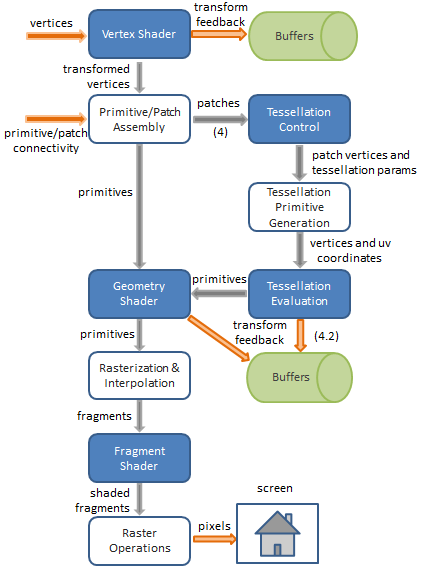
\includegraphics[height=0.47\textheight,keepaspectratio]{webgl_pipeline.png}
	\caption{WebGL's pipeline diagram~\cite{lighthouse3d_pipeline}}
	\label{fig:webgl_pipeline}
%\end{figure}
\end{wrapfigure}
\vspace{1pc}

Yet, it may seem that they are slightly similar they operate on totally different objects.
\newline Vertex shader operates only on each vertex individually not having a clue about remaining vertices.
\newline Fragment shader on the other hand operates on fragments\footnote{Data necessary to generate single pixel's worth of a drawing primitive in the frame buffer, e.g.: raster position, depth, interpolated attributes (color, texture coordinates, etc.), alpha value.}.
One can say that fragment shader takes care how pixels look in between the vertices (they interpolate the pixels' values following special rules defined in fragment shader).
Figure~\ref{fig:webgl_pipeline} shows WebGL's pipeline with vertex and fragment shaders marked there.

\clearpage

Vertex and fragment shaders have acces to OpenGL state, therefore they have access to state matrices like:
\begin{itemize}
\item Projection matrix (\texttt{uniform mat4 gl\_ProjectionMatrix}) - converts eye coordinates to clip coordinates,
\item Modelview matrix (\texttt{uniform mat4 gl\_ModelViewMatrix}) - result of multiplication of two matrices: 
\begin{itemize}
\item Model matrix which transforms object from object coordinates to world coordinates,
\item View matrix which converts world coordinates to eye coordinates. 
\end{itemize}
\end{itemize}

To completely be able to manipulate the vertex data one will need the incoming vertex that is fed to vertex shader.
This can be accessed by \texttt{attribute vec4 gl\_Vertex}
With those variables' (and many others fully listed in WebGL specification) one can manipulate the vertex data in vertex shader.
Fragment shader also has access to OpenGL state so using for instance \texttt{gl\_FragColor} it can set output fragment color.
Exemplar code of shaders is shown in Listing~\ref{lst:webgl_simple_shaders}. 

\begin{filecode}[label=lst:webgl_simple_shaders,language=HTML,caption=Exemplar implementation of vertex and fragment shaders written in GLSL ES.]
\lstinputlisting{./code/webgl_simple_shaders.html}
\end{filecode}

%============================================================

\clearpage
\section{Summary} 

OpenGL ES and WebGL are getting more and more popular with each day.
Even though we can find a lot of issue with them, like: 
\begin{itemize}
\item OpenGL ES - producers of mobile devices constantly striving to support the newest version of the standard in their drivers,
\item OpenGL ES - doesn't run on desktops, doesn't run on Web,
\item WebGL - getting mature and available on every modern browser but still needs some work to be as ubiquitous as OpenGL on desktops.
\end{itemize}
they allow us to use magnificent 3D effects in our hands usign mobile applcation or browsers.

Yet, one can frankly believe that WebGL is the best shot there is to bring 3D to every platform.
The Web has always been about: write once, run everywhere.

As long as browsers' developers will keep close to standards it is the best possibility to get 3D to each platform.

%============================================================

\clearpage
\label{Bibliography} 
%
\bibliographystyle{plain}
\footnotesize{ \bibliography{bibliography} }
% In that case, remember to run bibtex:
% latex template; bibtex template; latex template; latex template; 

%============================================================

\clearpage
\begin{appendices}

\section{Extending GLSurfaceView class to capture user input.}
\label{App:Appendix_A}
\begin{filecode}[label=lst:glsurfaceview_override]
\lstinputlisting{./code/opengles_glsurfaceview_override.java}
\end{filecode}

\end{appendices}

\end{document}